\documentclass{beamer}
\mode<presentation>
\usetheme{CambridgeUS}
\usepackage[russian]{babel}
\usepackage[utf8]{inputenc}
\usepackage[T2A]{fontenc}
\usepackage{sansmathaccent}

\usepackage{verbatim}
\usepackage{alltt}

\pdfmapfile{+sansmathaccent.map}
\title[Язык C]{Управление процессами, часть 6}
\author{Наумов Д.А., доц. каф. КТ}
\date[15.10.2019] {Операционные системы и системное программное обеспечение, 2019}

\begin{document}

%ТИТУЛЬНЫЙ СЛАЙД
\begin{frame}
  \titlepage
\end{frame}
  
%СОДЕРЖАНИЕ ЛЕКЦИИ
\begin{frame}
  \frametitle{Содержание лекции}
  \tableofcontents  
\end{frame}

\section{Концепция потоков в Linux}

\begin{frame}{Потоки}
\begin{block}{Потоки (threads)}
позволяют одновременно выполнять разные действия в контексте одной программы. 
\end{block}
Механизмы работы с потоками реализованы в \textit{Linux} в отдельной библиотеке \textit{Pthread}.

В рамках лекции будут рассмотрены следующие темы:
\begin{itemize}
\item Понятие потоков и их особенности.
\item Создание и завершение потока.
\item Синхронизация потоков.
\item Получение информации о потоках.
\item Обмен данными между потоками.
\end{itemize}
\end{frame}

\begin{frame}[fragile]
Когда один процесс вызывает fork(), в системе появляется другой процесс, который выполняет тот же код. Но данные, которыми манипулирует этот код, являются независимой копией данных процесса-родителя. 
\begin{alltt}
#include <stdio.h>
#include <unistd.h>
int main (void)\{
  int a = 10;
  pid\_t status = fork ();
  if (!status) \{
    a++; 
    printf ("Child's a=\%d", a);
    return 0;
  \}
  wait ();
  printf ("Parent's a=\%d", a);
  return 0;
\}
\end{alltt}
\end{frame}

\begin{frame}
\begin{block}{Процессы...}
\begin{itemize}
\item ... могут иметь общие данные, но для этого программисты обращаются к методам межпроцессного взаимодействия (interprocess communication). 
\item Межпроцессное взаимодействие подчас требует сложных манипуляций со стороны программиста.
\item В некоторых случаях плохо реализованное межпроцессное взаимодействие может стать мишенью для злоумышленников.
\end{itemize}
\end{block}
\begin{block}{Потоки}
\begin{itemize}
\item ...позволяют в рамках одной программы выполнять одновременно несколько
действий, используя при этом общие данные. 
\item ...выполняются так же, как и процессы, т. е. независимо
\end{itemize}
\end{block}
\end{frame}

\section{Создание потока}

\begin{frame}{Создание потока в Linux}
\begin{enumerate}
\item Создается функция, которая называется потоковой функцией.
\item При помощи функции pthread\_create() создается поток, в котором начинает параллельно остальной программе выполняться потоковая функция.
\item Вызывающая сторона продолжает выполнять какие-то действия, не дожидаясь завершения потоковой функции.
\end{enumerate}
Чтобы подключить библиотеку Pthread к программе, нужно передать компоновщику опцию -lpthread.
\end{frame}

\begin{frame}{Создание потока в Linux}
\begin{enumerate}
\item Создается функция, которая называется потоковой функцией.
\item При помощи функции pthread\_create() создается поток, в котором начинает параллельно остальной программе выполняться потоковая функция.
\item Вызывающая сторона продолжает выполнять какие-то действия, не дожидаясь завершения потоковой функции.
\end{enumerate}
Чтобы подключить библиотеку Pthread к программе, нужно передать компоновщику опцию -lpthread.
\begin{itemize}
\item каждый поток имеет идентификатор типа \textit{pthread\_t}
\item идентификаторы потока существуют локально в рамках текущего процесса.
\end{itemize}
\end{frame}

\begin{frame}{Создание потока в Linux}
\begin{figure}[h]
\centering
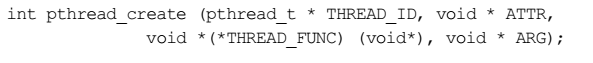
\includegraphics[scale=0.7]{images/lec08-pic01.png}
\end{figure}
Аргументы функции:
\begin{itemize}
\item THREAD\_ID - идентификатор нового потока (если таковой был создан).
\item ATTR - указание атрибутов потока. Если этот
аргумент равен NULL, то поток создается с атрибутами по умолчанию. 
\item PTHREAD\_FUNC - указатель на потоковую функцию. Это обычная функция, возвращающая бестиповый указатель (void*) и принимающая бестиповый указатель в качестве единственного аргумента.
\item ARG — указатель, содержащий аргументы потока. Если
потоковая функция не требует наличия аргументов, то в качестве ARG можно
указать NULL.
\end{itemize}
\end{frame}

\begin{frame}[fragile]{Пример}
\begin{itemize}
\item программа при запуске создает один поток, а функция pthread\_create() позволяет создавать дополнительные потоки;
\item основную программу следует трактовать как <<родительский поток>>;
\item если один из потоков завершает программу, то все остальные потоки тут же завершаются.
\end{itemize}
\begin{alltt}
void * any_func (void * args) \{
  fprintf (stderr, "Hello World");
  sleep (5);
  return NULL;
\}
int main (void)\{
  any_func (NULL);
  fprintf (stderr, "Goodbye World");
  while (1);
  return 0;
\}
\end{alltt}
\end{frame}

%\section{Завершение потока}
%\section{Ожидание потока}
%\section{Получение информации о потоке}
%\section{Отмена потока}
%\section*{Дополнительная инфомация}

\end{document}